\PassOptionsToPackage{unicode=true}{hyperref} % options for packages loaded elsewhere
\PassOptionsToPackage{hyphens}{url}
\PassOptionsToPackage{dvipsnames,svgnames*,x11names*}{xcolor}
%
\documentclass[ignorenonframetext,]{beamer}
\setbeamertemplate{caption}[numbered]
\setbeamertemplate{caption label separator}{: }
\setbeamercolor{caption name}{fg=normal text.fg}
\beamertemplatenavigationsymbolsempty
\usepackage{lmodern}
\usepackage{amssymb,amsmath}
\usepackage{ifxetex,ifluatex}
\usepackage{fixltx2e} % provides \textsubscript
\ifnum 0\ifxetex 1\fi\ifluatex 1\fi=0 % if pdftex
  \usepackage[T1]{fontenc}
  \usepackage[utf8]{inputenc}
  \usepackage{textcomp} % provides euro and other symbols
\else % if luatex or xelatex
  \usepackage{unicode-math}
  \defaultfontfeatures{Ligatures=TeX,Scale=MatchLowercase}
\fi
% use upquote if available, for straight quotes in verbatim environments
\IfFileExists{upquote.sty}{\usepackage{upquote}}{}
% use microtype if available
\IfFileExists{microtype.sty}{%
\usepackage[]{microtype}
\UseMicrotypeSet[protrusion]{basicmath} % disable protrusion for tt fonts
}{}
\IfFileExists{parskip.sty}{%
\usepackage{parskip}
}{% else
\setlength{\parindent}{0pt}
\setlength{\parskip}{6pt plus 2pt minus 1pt}
}
\usepackage{xcolor}
\usepackage{hyperref}
\hypersetup{
            pdftitle={Proportional Hazards Regression with Censored Data: Basics},
            pdfauthor={Dave Harrington},
            colorlinks=true,
            linkcolor=darkblue,
            citecolor=darkblue,
            urlcolor=darkblue,
            breaklinks=true}
\urlstyle{same}  % don't use monospace font for urls
\newif\ifbibliography
\usepackage{color}
\usepackage{fancyvrb}
\newcommand{\VerbBar}{|}
\newcommand{\VERB}{\Verb[commandchars=\\\{\}]}
\DefineVerbatimEnvironment{Highlighting}{Verbatim}{commandchars=\\\{\}}
% Add ',fontsize=\small' for more characters per line
\usepackage{framed}
\definecolor{shadecolor}{RGB}{248,248,248}
\newenvironment{Shaded}{\begin{snugshade}}{\end{snugshade}}
\newcommand{\AlertTok}[1]{\textcolor[rgb]{0.94,0.16,0.16}{#1}}
\newcommand{\AnnotationTok}[1]{\textcolor[rgb]{0.56,0.35,0.01}{\textbf{\textit{#1}}}}
\newcommand{\AttributeTok}[1]{\textcolor[rgb]{0.77,0.63,0.00}{#1}}
\newcommand{\BaseNTok}[1]{\textcolor[rgb]{0.00,0.00,0.81}{#1}}
\newcommand{\BuiltInTok}[1]{#1}
\newcommand{\CharTok}[1]{\textcolor[rgb]{0.31,0.60,0.02}{#1}}
\newcommand{\CommentTok}[1]{\textcolor[rgb]{0.56,0.35,0.01}{\textit{#1}}}
\newcommand{\CommentVarTok}[1]{\textcolor[rgb]{0.56,0.35,0.01}{\textbf{\textit{#1}}}}
\newcommand{\ConstantTok}[1]{\textcolor[rgb]{0.00,0.00,0.00}{#1}}
\newcommand{\ControlFlowTok}[1]{\textcolor[rgb]{0.13,0.29,0.53}{\textbf{#1}}}
\newcommand{\DataTypeTok}[1]{\textcolor[rgb]{0.13,0.29,0.53}{#1}}
\newcommand{\DecValTok}[1]{\textcolor[rgb]{0.00,0.00,0.81}{#1}}
\newcommand{\DocumentationTok}[1]{\textcolor[rgb]{0.56,0.35,0.01}{\textbf{\textit{#1}}}}
\newcommand{\ErrorTok}[1]{\textcolor[rgb]{0.64,0.00,0.00}{\textbf{#1}}}
\newcommand{\ExtensionTok}[1]{#1}
\newcommand{\FloatTok}[1]{\textcolor[rgb]{0.00,0.00,0.81}{#1}}
\newcommand{\FunctionTok}[1]{\textcolor[rgb]{0.00,0.00,0.00}{#1}}
\newcommand{\ImportTok}[1]{#1}
\newcommand{\InformationTok}[1]{\textcolor[rgb]{0.56,0.35,0.01}{\textbf{\textit{#1}}}}
\newcommand{\KeywordTok}[1]{\textcolor[rgb]{0.13,0.29,0.53}{\textbf{#1}}}
\newcommand{\NormalTok}[1]{#1}
\newcommand{\OperatorTok}[1]{\textcolor[rgb]{0.81,0.36,0.00}{\textbf{#1}}}
\newcommand{\OtherTok}[1]{\textcolor[rgb]{0.56,0.35,0.01}{#1}}
\newcommand{\PreprocessorTok}[1]{\textcolor[rgb]{0.56,0.35,0.01}{\textit{#1}}}
\newcommand{\RegionMarkerTok}[1]{#1}
\newcommand{\SpecialCharTok}[1]{\textcolor[rgb]{0.00,0.00,0.00}{#1}}
\newcommand{\SpecialStringTok}[1]{\textcolor[rgb]{0.31,0.60,0.02}{#1}}
\newcommand{\StringTok}[1]{\textcolor[rgb]{0.31,0.60,0.02}{#1}}
\newcommand{\VariableTok}[1]{\textcolor[rgb]{0.00,0.00,0.00}{#1}}
\newcommand{\VerbatimStringTok}[1]{\textcolor[rgb]{0.31,0.60,0.02}{#1}}
\newcommand{\WarningTok}[1]{\textcolor[rgb]{0.56,0.35,0.01}{\textbf{\textit{#1}}}}
\usepackage{graphicx,grffile}
\makeatletter
\def\maxwidth{\ifdim\Gin@nat@width>\linewidth\linewidth\else\Gin@nat@width\fi}
\def\maxheight{\ifdim\Gin@nat@height>\textheight\textheight\else\Gin@nat@height\fi}
\makeatother
% Scale images if necessary, so that they will not overflow the page
% margins by default, and it is still possible to overwrite the defaults
% using explicit options in \includegraphics[width, height, ...]{}
\setkeys{Gin}{width=\maxwidth,height=\maxheight,keepaspectratio}
% Prevent slide breaks in the middle of a paragraph:
\widowpenalties 1 10000
\raggedbottom
\setbeamertemplate{part page}{
\centering
\begin{beamercolorbox}[sep=16pt,center]{part title}
  \usebeamerfont{part title}\insertpart\par
\end{beamercolorbox}
}
\setbeamertemplate{section page}{
\centering
\begin{beamercolorbox}[sep=12pt,center]{part title}
  \usebeamerfont{section title}\insertsection\par
\end{beamercolorbox}
}
\setbeamertemplate{subsection page}{
\centering
\begin{beamercolorbox}[sep=8pt,center]{part title}
  \usebeamerfont{subsection title}\insertsubsection\par
\end{beamercolorbox}
}
\AtBeginPart{
  \frame{\partpage}
}
\AtBeginSection{
  \ifbibliography
  \else
    \frame{\sectionpage}
  \fi
}
\AtBeginSubsection{
  \frame{\subsectionpage}
}
\setlength{\emergencystretch}{3em}  % prevent overfull lines
\providecommand{\tightlist}{%
  \setlength{\itemsep}{0pt}\setlength{\parskip}{0pt}}
\setcounter{secnumdepth}{0}

% set default figure placement to htbp
\makeatletter
\def\fps@figure{htbp}
\makeatother


\usepackage{amsmath,verbatim}

\usepackage{fancyvrb}
\usepackage{manfnt}
\usepackage[normalem]{ulem}

%\usepackage[colorlinks=true]{hyperref}

\mode<presentation>{\usetheme{Malmoe}}

%\synctex=1

\setbeamertemplate{headline}{}


\setbeamerfont{footline}{size=\scriptsize}
\setbeamerfont{frametitle}{shape=\scshape}
\setbeamertemplate{itemize items}[circle]
\setbeamercovered{transparent}

\setbeamertemplate{navigation symbols}{}
\setbeamertemplate{footline}[frame number]{} 


\definecolor{forest}{rgb}{0, .5, 0}
\definecolor{brick}{rgb}{.5, 0, 0}
\definecolor{darkgreen}{rgb}{0, .5, 0}
\definecolor{darkred}{rgb}{.7, .15, .15}
\definecolor{darkblue}{rgb}{0, 0, .5}
\definecolor{Green}{rgb}{0.2,1,0.2}


\newcommand{\R}{\textsf{R}}
\newcommand{\RStudio}{\textsl{R Studio}}
\newcommand{\var}{\mbox{Var}}
\newcommand{\Cov}{\mbox{Cov}}
\newcommand{\Cor}{\mbox{Cor}}
\newcommand{\cip}{\mbox{$\perp\!\!\!\perp$}}
\newcommand{\bpsi}{\mbox{\boldmath$\psi$}}
\newcommand{\bbeta}{\mbox{\boldmath$\beta$}}
\newcommand{\bhat}{\mbox{\boldmath$\hat\beta$}}
\newcommand{\btheta}{\mbox{\boldmath$\theta$}}
\newcommand{\beeta}{\mbox{\boldmath$\eta$}}
\newcommand{\bfeta}{\mbox{\boldmath$\eta$}}
\newcommand{\bpsinot}{\mbox{\boldmath{$\psi_0$}}}
\newcommand{\bZ}{\bf Z}

%\usepackage[english]{babel}
\usepackage{lmodern}
\renewcommand\ttfamily{\usefont{T1}{lmtt}{m}{n}}

%\usepackage{palatino}
\usepackage[T1]{fontenc}
%\usepackage[lmodern]{babel}

% make all tt fonts bold to look more like Verbatim
\renewcommand\ttfamily{\usefont{T1}{lmtt}{m}{n}}

% Comment these out if you don't want a slide with just the
% part/section/subsection/subsubsection title:
\AtBeginPart{
  \let\insertpartnumber\relax
  \let\partname\relax
  \frame{\partpage}
}
\AtBeginSection{
  \let\insertsectionnumber\relax
  \let\sectionname\relax
  \frame{\sectionpage}
}
\AtBeginSubsection{
  \let\insertsubsectionnumber\relax
  \let\subsectionname\relax
  \frame{\subsectionpage}
}

\begin{comment}

%reduces space between code chunk and output
\usepackage{etoolbox}
\setlength{\parskip}{0pt}
\setlength{\OuterFrameSep}{0pt}
\makeatletter
\preto{\@verbatim}{\topsep=-10pt \partopsep=10pt }
\makeatother

\end{comment}

\title{Proportional Hazards Regression with Censored Data: Basics}
\author{Dave Harrington}
\date{May 14 - 18, 2018}

\begin{document}
\frame{\titlepage}

\begin{frame}
\tableofcontents[hideallsubsections]
\end{frame}
\hypertarget{introduction}{%
\section{Introduction}\label{introduction}}

\begin{frame}[fragile]{%
\protect\hypertarget{regression-models-for-survival-data}{%
Regression models for survival data}}

These notes focus on proportional hazards regression models.

\emph{Proportional Hazards (PH) models}\\
\[   \lambda(t;{\bf Z}) = \lambda_0(t) \Psi({\bf Z}) \]

\begin{verbatim}
- The second term is usually written $\Psi(Z) =  e^{\beta Z}$.

- Suppose $Z=1$ for treated subjects and $Z=0$ for untreated subjects.  The hazard is increased by a factor of $e^\beta$ for treated subjects versus untreated subjects.
     
- This is a *semi-parametric* model.
\end{verbatim}

\end{frame}

\begin{frame}{%
\protect\hypertarget{other-regression-models-for-survival-data}{%
Other regression models for survival data}}

\emph{Accelerated Failure Time (AFT) models}\\
\[  \log(T) = \mu + {\bbeta} {\bf Z} +  \sigma W,\]

\begin{itemize}
\item
  \(W\) is an \emph{error term}.
\item
  Typically (but not always), there is a \emph{parametric} model for
  \(W\):

  \begin{itemize}
  \tightlist
  \item
    exponential, Weibull, gamma, or log-normal
  \end{itemize}
\end{itemize}

\emph{Additive Hazards Regression models} \[
   \lambda(t; Z(t) = \beta_0(t) + \sum_{k=1}^p \beta_k(t) Z_k(t)
\]

Klein \& Moeschberger have excellent treatments of both of these models

\end{frame}

\begin{frame}{%
\protect\hypertarget{covariates}{%
Covariates}}

In general, \({\bf Z}\) is a \(p\)-dimensional vector of covariates.
\({\bf Z}\) may include

\begin{itemize}
\item
  continuous factors (e.g., age, blood pressure)
\item
  discrete factors (e.g., sex, marital status)
\item
  possible interactions (e.g., age by sex interaction)
\end{itemize}

Two covariates, \(A\) and \(B\), interact if

\begin{itemize}
\item
  hazard of death depends on the combination of \(A\) and \(B\)
\item
  best to only include interactions if the corresponding main effects
  are also included
\end{itemize}

\end{frame}

\begin{frame}{%
\protect\hypertarget{covariates-1}{%
Covariates\ldots}}

A categorical covariate \(A\) with \(a\) levels is usually modeled with

\begin{itemize}
\item
  \((a-1)\) binary
  variables\footnote{These are sometimes called dummy variables or 0-1 variables.}
  (\(U_1,U_2,\ldots,U_a\)) such that \(U_j=1 \, \, \mbox{ if } A=j\).
\item
  Then,
  \[\lambda_i(t)=\lambda_0(t)\exp(\beta_2 U_2+\beta_3 U_3+\cdots+\beta_a U_a)\]
\item
  In the above model, the subgroup with \(A=1\) or \(U_1=1\) is the
  reference group.
\end{itemize}

Alternatively, in \textsf{R}, categorical covariates can (and should) be
stored or converted to \emph{factor} variables.

\end{frame}

\hypertarget{the-cox-proportional-hazards-ph-model}{%
\section{The Cox proportional hazards (PH)
model}\label{the-cox-proportional-hazards-ph-model}}

\begin{frame}{%
\protect\hypertarget{the-cox-model}{%
The Cox model}}

The Cox (1972) proportional hazards model is given by

\[\lambda(t;{\bf Z}) = \lambda_0(t) \exp(\beta {\bf Z}).\]

This is the most common model used for survival
data.\footnote{Some books use $h(t;{\bf X})$ as their standard notation
instead of $\lambda(t;{\bf Z})$.}

\begin{itemize}
\item
  Natural interpretation
\item
  Allows for flexible choice of covariates
\item
  Fairly easy to fit
\item
  Robust software exists in nearly all standard packages
\end{itemize}

\small

References

\begin{itemize}
\item
  Collett, Chapter 3
\item
  Cox and Oakes, Chapter 7
\item
  Klein and Moeschberger, Chapters 8 \& 9
\end{itemize}

\end{frame}

\begin{frame}{%
\protect\hypertarget{why-the-name-proportional-hazards}{%
Why the name proportional hazards?}}

Suppose in two groups, \(Z=1\) for treated and \(Z=0\) for control. If

\begin{itemize}
\item
  \(\lambda_1(t)\) is the hazard rate for the treated group and
\item
  \(\lambda_0(t)\) is the hazard for control, then
\end{itemize}

\[ \lambda_1(t) = \lambda(t;Z=1) = \lambda_0(t) \exp(\beta Z) = \lambda_0(t) \exp(\beta)\]

The ratio of the two hazards is a constant, \(\phi\), which does not
depend on time; \(\phi\) is referred to as the \emph{hazard ratio}.
\[\phi = \frac{\lambda_1(t)}{\lambda_0(t)} = e^{\beta} \]

The hazards of the two groups remain proportional over time.

\end{frame}

\begin{frame}{%
\protect\hypertarget{the-baseline-hazard-function}{%
The baseline hazard function}}

In general, \(\lambda_0(t)\) is called the \emph{baseline hazard
function}.

\begin{itemize}
\tightlist
\item
  It is the underlying hazard for subjects with all covariates
  \(Z_1, \ldots ,Z_p\) equal to 0 (i.e., the “reference group”).
\end{itemize}

General form of the PH model:
\[\lambda(t;{\bf Z}) =  \lambda_0(t) \exp(\beta_1 Z_1 + \beta_2 Z_2 + \cdots + \beta_p Z_p) \]

When all of the \(Z_j\)’s equal 0: \begin{align*}
\lambda(t;{\bf Z} = 0) &= \lambda_0(t) \exp(\beta_1(0) + \beta_2(0) + \cdots + \beta_p(0)\\
&= \lambda_0(t)
\end{align*}

\end{frame}

\begin{frame}{%
\protect\hypertarget{role-of-the-explanatory-variables}{%
Role of the explanatory variables}}

In the general case, the \(i\)-th individual has a set of covariates in
a column vector \({\bf Z}_i=(Z_{1i}, Z_{2i},..., Z_{pi})\). The hazard
rate is modeled as some multiple of the baseline hazard:
\[ \lambda_i(t;{\bf Z}_i) = \lambda_0(t) \exp(\beta_1 Z_{1i} + \cdots + \beta_p Z_{pi})\]

\end{frame}

\begin{frame}{%
\protect\hypertarget{why-the-name-proportional-hazards-again}{%
Why the name proportional hazards? (again!)}}

The log of the hazard ratio for the \(i\)-th individual compared to the
reference group can be written as
\[\log \left(\frac{\lambda_i(t)}{\lambda_0(t)}\right) 
= \beta_1 Z_{1i} + \beta_2 Z_{2i} + \cdots + \beta_p Z_{pi}. \]

The Cox PH model is a linear model for the log of the hazard ratio.

\begin{itemize}
\item
  Surprisingly, the parameter \(\beta\) can be estimated without having
  to make assumptions about \(\lambda_0(t)\).
\item
  This is the reason for the terminology \emph{semi-parametric}.
\end{itemize}

Estimating equations coming after an example.

\end{frame}

\begin{frame}{%
\protect\hypertarget{example-rossi-recidivism-data-survival-curves}{%
Example: Rossi recidivism data, survival curves}}

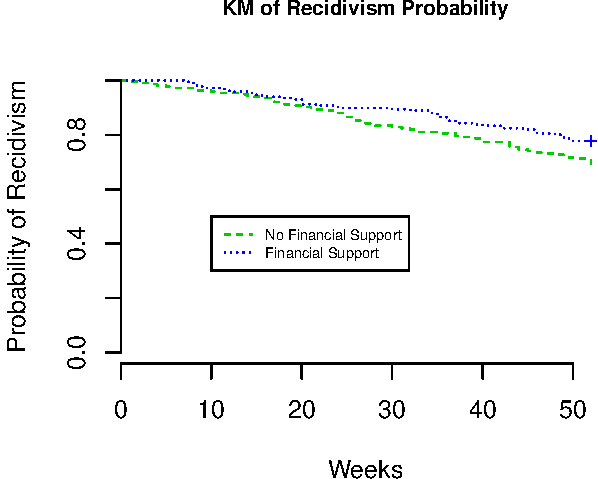
\includegraphics{unit_04_ph_reg_basics_files/figure-beamer/unnamed-chunk-1-1.pdf}

\end{frame}

\begin{frame}{%
\protect\hypertarget{rossi-data-cumulative-hazards}{%
Rossi data, cumulative hazards}}

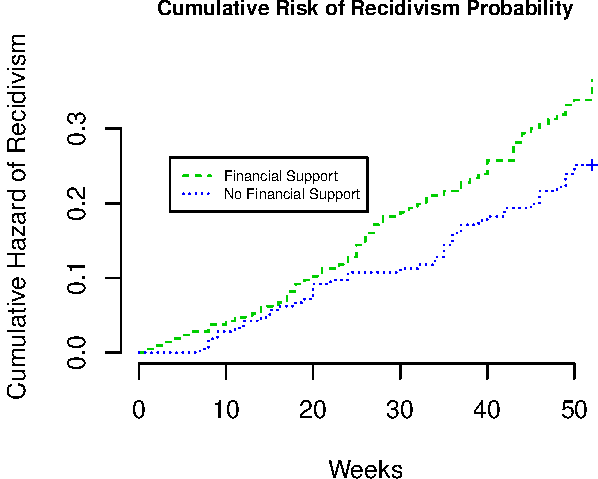
\includegraphics{unit_04_ph_reg_basics_files/figure-beamer/unnamed-chunk-2-1.pdf}

\end{frame}

\begin{frame}{%
\protect\hypertarget{example-rossi-recidivism-data}{%
Example: Rossi recidivism data \ldots}}

Let

\begin{itemize}
\item
  \(T\) be time to recidivism (the variable \texttt{week})
\item
  \(Z\) denote randomization to financial incentive (the variable
  \texttt{fin})
\end{itemize}

Estimate and interpret the model \[
\lambda(t; Z) = \lambda_0 \exp(\beta Z)
\]

\end{frame}

\begin{frame}[fragile]{%
\protect\hypertarget{example-rossi-recidivism-data-1}{%
Example: Rossi recidivism data \ldots}}

\small

\begin{Shaded}
\begin{Highlighting}[]
\KeywordTok{library}\NormalTok{(survival)}
\KeywordTok{library}\NormalTok{(eventtimedata)}
\KeywordTok{data}\NormalTok{(rossi)}
\KeywordTok{coxph}\NormalTok{(}\KeywordTok{Surv}\NormalTok{(week, arrest) }\OperatorTok{~}\StringTok{ }\NormalTok{fin, }\DataTypeTok{data =}\NormalTok{ rossi)}
\end{Highlighting}
\end{Shaded}

\begin{verbatim}
## Call:
## coxph(formula = Surv(week, arrest) ~ fin, data = rossi)
## 
##          coef exp(coef) se(coef)     z     p
## finyes -0.369     0.691    0.190 -1.95 0.052
## 
## Likelihood ratio test=3.84  on 1 df, p=0.0501
## n= 432, number of events= 114
\end{verbatim}

\normalsize

\end{frame}

\begin{frame}{%
\protect\hypertarget{interpretation}{%
Interpretation}}

The term \texttt{coef} is the \(\beta\) coefficient for \texttt{fin}.

\begin{itemize}
\item
  There are 114 events (re-arrests) in 432 cases.
\item
  The value -0.369 implies that the hazard for re-arrest is lower in the
  financial incentive group by a factor of \(\exp(-0.369) = 0.691\).
\item
  The standard error for the coefficient is 0.190.
\item
  The Wald statistic \(p\)-value for a test of \(H_0: \beta = 0\) is
  0.052.

  \begin{itemize}
  \item
    The Wald test statistic used to test \(H_0: \beta = 0\) is given by
    \[\frac{\widehat{\beta}}{\text{s.e.}(\widehat{\beta})}\]
  \item
    The likelihood ratio (LR) test of the same hypothesis has a similar
    result. Definition of the LR test coming later.
  \end{itemize}
\end{itemize}

There is \emph{no} information about \(\lambda_0(t)\) in the output.
That follows from the method of estimation.

\end{frame}

\begin{frame}{%
\protect\hypertarget{likelihood-estimation-for-the-ph-model}{%
Likelihood estimation for the PH model}}

There have been several derivations of the likelihood used for the PH
model.

Cox (1972) derived a \emph{partial likelihood}.

Suppose the data for an individual \(i\) are
\((X_i, \delta_i, {\bf Z}_i)\), where

\begin{itemize}
\item
  \(X_i\) is a censored failure time random variable
\item
  \(\delta_i\) is the failure/censoring indicator (1=fail, 0=censor)
\item
  \({\bf Z}_i\) represents a set of covariates
\end{itemize}

The covariates may be continuous, discrete, or time-varying.

Suppose there are \(K\) distinct failure times, and let
\(\tau_1,....\tau_K\) represent the \(K\) ordered, distinct death times.

For now, assume there are no tied death times.

\end{frame}

\begin{frame}{%
\protect\hypertarget{the-partial-likelihood}{%
The partial likelihood}}

Let \({\cal R}(t) = \{ i: x_i \ge t \}\) denote the set of individuals
who are ``at risk’’ for failure at time \(t\).

Notation for risk sets:

\begin{itemize}
\item
  \({\cal R}(\tau_j)\) is the risk set at the \(j\)-th failure time.
\item
  \({\cal R}(X_i)\) is the risk set at the failure time of individual
  \(i\).
\item
  \(r_j\) is the number of individuals in \({\cal R}(\tau_j)\), while
  \({\cal R}(\tau_j)\) identifies the subjects at risk.
\end{itemize}

Intuitively, the partial likelihood is a product over the set of
observed failure times of the conditional probabilities of seeing the
observed deaths, given the set of individuals at risk at those times.

\end{frame}

\begin{frame}{%
\protect\hypertarget{the-partial-likelihood-1}{%
The partial likelihood \ldots}}

At each failure time \(\tau_j\), the contribution to the likelihood is:
\begin{align*}
 L_j(\bbeta)   &= 
     P(\mbox{individual $j$ fails} | 1 \mbox{ failure from }{\cal R}(\tau_j) )\\[2ex]
 &=  \frac
  {  P(\mbox{individual } j \mbox{ fails} | \mbox{ at risk at } \tau_j)}
       {\sum_{\ell \in {\cal R}(\tau_j)}
      P(\mbox{individual } \ell \mbox{ fails} | \mbox{ at risk at } \tau_j) }
\\[2ex]
 &= 
    \frac
  {  \lambda(\tau_j; {\bf Z}_j) }  {\sum_{\ell \in {\cal R}(\tau_j)}
       \lambda(\tau_j; {\bf Z}_\ell) } \\
\end{align*}

\end{frame}

\begin{frame}{%
\protect\hypertarget{the-partial-likelihood-2}{%
The partial likelihood \ldots}}

Under the PH assumption,
\(\lambda(t; {\bf Z}) = \lambda_0(t) e^{\bbeta \bf Z}\), so

\begin{align*}
 L^{partial}(\beta)  
 &= \prod_{j=1}^{K} \frac
  {  \lambda_0(\tau_j) e^{\bbeta {\bf Z}_j } }   {\sum_{\ell \in {\cal R}(\tau_j)}
        \lambda_0(\tau_j) e^{\bbeta {\bf Z}_\ell} } \\[2ex]
 &= \prod_{j=1}^{K} \frac
  {   e^{\bbeta {\bf Z}_j } }   {\sum_{\ell \in {\cal R}(\tau_j)}
        e^{\bbeta {\bf Z}_\ell} } \\
\end{align*}

This is equivalent to the partial likelihood as defined by Cox
\[L^{partial}(\beta) = \prod_{j=1}^{n} \left[\frac{e^{\beta {\bf Z}_j}}{
\sum_{\ell\in {\cal R}(X_j)} e^{\beta {\bf Z}_\ell}}\right]^{\delta_i} \]

Contributions to the partial likelihood occur only at failure times.

\end{frame}

\begin{frame}{%
\protect\hypertarget{a-simple-example}{%
A simple example}}

\begin{center}
\begin{tabular}{cccc}
\hline
individual & ~~$X_i$~~ &  ~~$\delta_i$~~ & ~~$Z_i$~~ \\ 
\hline
1  &  ~9 & 1 & 4 \\ 
2  &  ~8 & 0 & 5 \\ 
3  &  ~6 & 1 & 7 \\ 
4  &  10 & 1 & 3 \\ \hline
\end{tabular}
\end{center}

Now compile the pieces that go into the partial likelihood contributions
at each failure time \ldots

\end{frame}

\begin{frame}{%
\protect\hypertarget{a-simple-example-1}{%
A simple example \ldots}}

\footnotesize
\begin{center}
\begin{tabular}{ccccc}
    & ordered & \\
    & failure & & & Likelihood contribution\\
$j$ & time $X_i$ &  ${\cal R}(X_i)$  & ~~~$i_j$~~~ & 
$\left[e^{\beta Z_i}/
\sum_{j\in {\cal R}(X_i)} e^{\beta Z_j}\right]^{\delta_i}$ \\ \hline 
~~\\
1 & ~6 & \{1,2,3,4\} & 3 & 
$e^{7\beta}/[e^{4\beta} + e^{5\beta} + e^{7\beta} + e^{3\beta}]$\\[3ex]
2 & ~8 & \{1,2,4\} & 2 & $e^{5\beta}/[e^{4\beta} + e^{5\beta} + e^{3\beta}]^0 = 1$ \\[3ex]
3 & ~9 & \{1,4\} & 1 & 
$e^{4\beta}/[e^{4\beta} + e^{3\beta}]$\\[3ex]
4 & 10 & \{4\} & 4 & 
$e^{3\beta}/e^{3\beta}=1$ \\ \\ \hline 
\end{tabular}
\end{center}

The partial likelihood is the product of these four terms.

The estimate for \(\beta\) is the value \(\widehat{\beta}\) that
maximizes the partial likelihood.

\end{frame}

\begin{frame}[fragile]{%
\protect\hypertarget{a-more-realistic-example-rossi-data}{%
A more realistic example: Rossi data}}

\small

\begin{Shaded}
\begin{Highlighting}[]
\KeywordTok{library}\NormalTok{(survival)}
\KeywordTok{library}\NormalTok{(eventtimedata)}
\KeywordTok{data}\NormalTok{(rossi)}
\KeywordTok{coxph}\NormalTok{(}\KeywordTok{Surv}\NormalTok{(week, arrest) }\OperatorTok{~}\StringTok{ }\NormalTok{fin }\OperatorTok{+}\StringTok{ }\NormalTok{age }\OperatorTok{+}\StringTok{ }\NormalTok{race }\OperatorTok{+}\StringTok{ }\NormalTok{mar, }
      \DataTypeTok{data =}\NormalTok{ rossi)}
\end{Highlighting}
\end{Shaded}

Output next slide.

We will discuss interpretation in class.

\end{frame}

\begin{frame}[fragile]{%
\protect\hypertarget{a-more-realistic-example-rossi-data-1}{%
A more realistic example: Rossi data}}

\footnotesize

\begin{verbatim}
## Call:
## coxph(formula = Surv(week, arrest) ~ fin + age + race + mar, 
##     data = rossi)
## 
##                  coef exp(coef) se(coef)     z      p
## finyes         -0.351     0.704    0.190 -1.84 0.0654
## age            -0.065     0.937    0.021 -3.10 0.0019
## raceother      -0.244     0.784    0.306 -0.80 0.4258
## marnot married  0.508     1.663    0.373  1.36 0.1735
## 
## Likelihood ratio test=21.2  on 4 df, p=0.000289
## n= 432, number of events= 114
\end{verbatim}

\normalsize

\end{frame}

\begin{frame}{%
\protect\hypertarget{categorical-variables-coded-as-numeric}{%
Categorical variables coded as numeric}}

Education (\texttt{educ}) is coded on the dataset as an integer variable
with values 2 - 6.\footnote{See the documentation for definitions.}

The next two slides show two models.

\begin{itemize}
\item
  Model with \texttt{educ} fitted as a numeric variable
\item
  Model with \texttt{educ} converted to a factor variable
\end{itemize}

\end{frame}

\begin{frame}[fragile]{%
\protect\hypertarget{categorical-variables-coded-as-numeric-1}{%
Categorical variables coded as numeric \ldots}}

\small

\begin{Shaded}
\begin{Highlighting}[]
\KeywordTok{library}\NormalTok{(survival)}
\KeywordTok{library}\NormalTok{(eventtimedata)}
\KeywordTok{data}\NormalTok{(rossi)}
\KeywordTok{coxph}\NormalTok{(}\KeywordTok{Surv}\NormalTok{(week, arrest) }\OperatorTok{~}\StringTok{ }\NormalTok{fin }\OperatorTok{+}\StringTok{ }\NormalTok{educ, }\DataTypeTok{data =}\NormalTok{ rossi)}
\end{Highlighting}
\end{Shaded}

\begin{verbatim}
## Call:
## coxph(formula = Surv(week, arrest) ~ fin + educ, data = rossi)
## 
##          coef exp(coef) se(coef)     z     p
## finyes -0.351     0.704    0.190 -1.85 0.065
## educ   -0.256     0.774    0.120 -2.14 0.033
## 
## Likelihood ratio test=8.7  on 2 df, p=0.0129
## n= 432, number of events= 114
\end{verbatim}

\end{frame}

\begin{frame}[fragile]{%
\protect\hypertarget{categorical-variables-coded-as-numeric-be-careful}{%
Categorical variables coded as numeric: be careful \ldots}}

\footnotesize

\begin{Shaded}
\begin{Highlighting}[]
\KeywordTok{library}\NormalTok{(survival)}
\KeywordTok{library}\NormalTok{(eventtimedata)}
\KeywordTok{data}\NormalTok{(rossi)}
\KeywordTok{coxph}\NormalTok{(}\KeywordTok{Surv}\NormalTok{(week, arrest) }\OperatorTok{~}\StringTok{ }\NormalTok{fin }\OperatorTok{+}\StringTok{ }\KeywordTok{as.factor}\NormalTok{(educ), }\DataTypeTok{data =}\NormalTok{ rossi)}
\end{Highlighting}
\end{Shaded}

\begin{verbatim}
## Call:
## coxph(formula = Surv(week, arrest) ~ fin + as.factor(educ), data = rossi)
## 
##                    coef exp(coef) se(coef)     z     p
## finyes           -0.402     0.669    0.190 -2.11 0.035
## as.factor(educ)3  0.841     2.318    0.514  1.64 0.102
## as.factor(educ)4  0.459     1.583    0.537  0.86 0.393
## as.factor(educ)5 -0.187     0.830    0.671 -0.28 0.781
## as.factor(educ)6 -0.534     0.586    1.119 -0.48 0.633
## 
## Likelihood ratio test=16.3  on 5 df, p=0.00605
## n= 432, number of events= 114
\end{verbatim}

\end{frame}

\begin{frame}{%
\protect\hypertarget{categorical-variables-coded-as-numeric-2}{%
Categorical variables coded as numeric \dots}}

The second model is preferable.

\begin{itemize}
\tightlist
\item
  Why?
\end{itemize}

To assess whether \texttt{educ} signficantly adds to the second model:

\begin{itemize}
\item
  Conduct a likelihood ratio test using the change in log(partial
  likelihood) when \texttt{educ} is added to a model with \texttt{fin}
\item
  Some theory is needed first.
\end{itemize}

\end{frame}

\hypertarget{the-partial-likelihood-3}{%
\section{The partial likelihood}\label{the-partial-likelihood-3}}

\begin{frame}{%
\protect\hypertarget{review-of-likelihood-based-inference}{%
Review of likelihood-based inference}}

Suppose

\begin{itemize}
\item
  \(L(\beta)\) is the likelihood for a one dimensional parameter
  \(\beta\) in a model, and
\item
  \(\ell(\beta) = \log(L(\beta))\)
\end{itemize}

Tests of \(H_0:\beta = \beta_0\) can be based on three asymptotically
equivalent statistics.

\end{frame}

\begin{frame}{%
\protect\hypertarget{review-of-likelihood-based-inference-1}{%
Review of likelihood-based inference\ldots}}

Wald statistic:

\[  
  \frac{\widehat{\beta} - \beta_0}{\text{s.e.}(\widehat{\beta})} \sim N(0,1).
\]

Log-likelihood ratio statistic:

\[
-2 \left[\log(L(\widehat{\beta})) - \log(L(\beta_0))\right] \sim \chi^2 (1).
\]

Score test statistic:

\[
  U(\beta_0) =  \frac{\partial}{\partial \beta}\Bigr|_{\beta = \beta_0} \ell(\beta) \sim N(0,1)
\]

All have multivariate versions for \(p\)-dimensional parameter vectors
\(\bbeta\), not shown here.

\end{frame}

\begin{frame}{%
\protect\hypertarget{review-of-likelihood-based-inference-2}{%
Review of likelihood-based inference\ldots}}

The statistical literature has results on which test is preferred, but
that is not covered here.

The tests are usually similar enough that choice of a statistic is based
on convenience.

Example coming later.

\end{frame}

\begin{frame}{%
\protect\hypertarget{partial-likelihood-inference}{%
Partial likelihood inference}}

Inference can be conducted by treating the partial likelihood as though
it satisfies all the regular likelihood properties.

The \emph{log(partial likelihood)} is: \begin{align*}
\ell(\bbeta)   &= \log \left[ \prod_{j=1}^{n}    \frac 
  {   e^{\bbeta {\bf Z}_j } }   {\sum_{\ell \in {\cal R}(\tau_j)}
        e^{\bbeta {\bf Z}_\ell} } \right]^{\delta_j}  \\
       &= \log \left[ \prod_{j=1}^{K}    \frac 
  {   e^{\bbeta {\bf Z}_j } }   {\sum_{\ell \in {\cal R}(\tau_j)}
        e^{\bbeta {\bf Z}_\ell} } \right]  \\
 &= \sum_{j=1}^{K}   \left[ \beta {\bf Z}_j  - 
      \log [\sum_{\ell \in {\cal R}(\tau_j)} e^{\bbeta {\bf Z}_\ell}] \right]  \\
 &=  \sum _{j=1}^{K}  l_j (\bbeta) 
\end{align*} where \(l_j\) is the log-partial likelihood contribution at
the \(j\)-th ordered death time.

\end{frame}

\begin{frame}{%
\protect\hypertarget{partial-likelihood-inference-1}{%
Partial likelihood inference}}

Suppose there is only one covariate (\(\beta\) is one-dimensional):

The \emph{partial likelihood score equations} are:
\[   U(\beta) = \frac{\partial}{\partial \beta} \ell(\beta) = 
    \sum_{j=1}^{n}   \delta_j \left[   Z_j  -  
      \frac{ \sum_{\ell \in {\cal R}(\tau_j)}  Z_\ell e^{\beta  Z_\ell} }
          { \sum_{\ell \in {\cal R}(\tau_j)}   e^{\beta  Z_\ell} } \right]
\]

\(U(\beta)\) is a sum of \emph{observed} minus \emph{expected} values:

\[   U(\beta) = \frac{\partial}{\partial \beta} \ell(\beta) = 
    \sum_{j=1}^{n}  \delta_j 
    (   Z_j  -  \overline{Z}_j  )  \] where \(\overline{Z}_j\) is the
\emph{weighted average} of Z over the individuals in the risk set at
time \(\tau_j\).

Note that \(\beta\) is involved through the term \(\overline{Z}_j\).

The maximum partial likelihood estimators can be found by solving
\(U(\beta) =0\).

\end{frame}

\begin{frame}{%
\protect\hypertarget{partial-likelihood-inference-2}{%
Partial Likelihood inference \ldots}}

Analogous to standard likelihood theory, it can be shown that
\[   \frac{(\widehat{\beta}-\beta)}{\text{s.e.}(\hat{\beta})} \sim N(0,1) \]
The variance of \(\widehat{\beta}\) can be obtained by inverting the
second derivative of the partial likelihood,
\[   \text{var}(\widehat{\beta}) \sim \left[
     -\frac{\partial^2}{\partial \beta^2} \ell(\beta)\right]^{-1}   \]
From the above expression for \(U(\beta)\): \[  
\frac{\partial^2}{\partial \beta^2} \ell(\beta) = 
 \sum_{j=1}^{n}   \delta_j \left[     -  
      \frac{ \sum_{\ell \in {\cal R}(\tau_j)}  (   Z_j  -  \bar{Z}_j  )^2
        e^{\beta  Z_\ell} }
          { \sum_{\ell \in {\cal R}(\tau_j)}  e^{\beta  Z_\ell} } \right]
\]

The actual variance of \(\widehat\beta\) is a function of the unknown
\(\beta\).

The \emph{observed} information is calculated by substituting the
partial likelihood estimate of \(\beta\) into the above formula for the
variance.

\end{frame}

\begin{frame}[fragile]{%
\protect\hypertarget{example-rossi-recidivism-data-2}{%
Example: Rossi recidivism data}}

Suppose the primary interest is in evaluating the effect of financial
incentive on changing the rate of recidivism, after adjusting for

\begin{itemize}
\tightlist
\item
  \texttt{age}, \texttt{race}, \texttt{mar}, \texttt{educ}
\end{itemize}

\small

\begin{Shaded}
\begin{Highlighting}[]
\KeywordTok{library}\NormalTok{(survival)}
\KeywordTok{library}\NormalTok{(eventtimedata)}
\KeywordTok{data}\NormalTok{(rossi)}
\KeywordTok{coxph}\NormalTok{(}\KeywordTok{Surv}\NormalTok{(week, arrest) }\OperatorTok{~}\StringTok{ }\NormalTok{fin }\OperatorTok{+}\StringTok{ }\NormalTok{age }\OperatorTok{+}\StringTok{ }\NormalTok{race }\OperatorTok{+}\StringTok{ }\NormalTok{mar }
      \OperatorTok{+}\StringTok{ }\KeywordTok{as.factor}\NormalTok{(educ), }\DataTypeTok{data =}\NormalTok{ rossi)}
\end{Highlighting}
\end{Shaded}

\normalsize

\end{frame}

\begin{frame}[fragile]{%
\protect\hypertarget{example-rossi-recidivism-data-3}{%
Example: Rossi recidivism data \ldots}}

\footnotesize

\begin{verbatim}
## Call:
## coxph(formula = Surv(week, arrest) ~ fin + age + race + mar + 
##     as.factor(educ), data = rossi)
## 
##                     coef exp(coef) se(coef)     z      p
## finyes           -0.3853    0.6802   0.1921 -2.01 0.0448
## age              -0.0555    0.9460   0.0211 -2.63 0.0087
## raceother        -0.3405    0.7114   0.3103 -1.10 0.2725
## marnot married    0.4715    1.6024   0.3751  1.26 0.2087
## as.factor(educ)3  0.6344    1.8858   0.5200  1.22 0.2225
## as.factor(educ)4  0.2362    1.2665   0.5420  0.44 0.6629
## as.factor(educ)5 -0.2572    0.7732   0.6724 -0.38 0.7021
## as.factor(educ)6 -0.5018    0.6054   1.1219 -0.45 0.6546
## 
## Likelihood ratio test=30  on 8 df, p=0.000212
## n= 432, number of events= 114
\end{verbatim}

\end{frame}

\begin{frame}{%
\protect\hypertarget{interpretation-1}{%
Interpretation}}

\begin{itemize}
\item
  Financial incentive appears to significantly reduce the rate of
  recidivism by approximately 32\% (adjusted hazard ratio 0.68).
\item
  The likelihood ratio (\emph{LR}) test (30 on 8 df) is highly
  significant; this full set of covariates is significantly associated
  with the rate of recidivism.

  \begin{itemize}
  \item
    Formally, the \emph{LR} test is a test of \(H_0:\bbeta = {\bf 0}\).
  \item
    The statistic is
    \(-2\left[\ell(\widehat{\bbeta}) - \ell({\bf 0})\right]\).
  \item
    It has 8 df, since the difference in the number of parameters
    between the full model and the null model is 8.
  \item
    The LR test is analogous to an \(F\)-test in linear regression
  \end{itemize}
\end{itemize}

\end{frame}

\begin{frame}[fragile]{%
\protect\hypertarget{interpretation-2}{%
Interpretation\ldots}}

\begin{itemize}
\item
  Age is significantly associated with recidivsm: younger participants
  have a rate that is about 5\% lower.

  \begin{itemize}
  \tightlist
  \item
    Why is the \(p\)-value so small when the effect size is also very
    small?
  \end{itemize}
\item
  Confidence intervals for the adjusted hazard ratio for age can be
  found by calculating a confidence interval for \(\widehat{\beta}\)
  then
  exponentiating.\footnote{Possible to do this entirely within \textsf{R} without any `hand' substitutions; method shown later.}
\end{itemize}

\small

\begin{Shaded}
\begin{Highlighting}[]
\NormalTok{beta.hat =}\StringTok{ }\FloatTok{-0.0555}\NormalTok{; se.beta.hat =}\StringTok{ }\FloatTok{0.0211}
\NormalTok{m =}\StringTok{ }\FloatTok{1.96}\OperatorTok{*}\NormalTok{se.beta.hat}
\KeywordTok{exp}\NormalTok{(beta.hat }\OperatorTok{-}\StringTok{ }\NormalTok{m); }\KeywordTok{exp}\NormalTok{(beta.hat }\OperatorTok{+}\StringTok{ }\NormalTok{m)}
\end{Highlighting}
\end{Shaded}

\begin{verbatim}
## [1] 0.90769
\end{verbatim}

\begin{verbatim}
## [1] 0.98596
\end{verbatim}

\end{frame}

\begin{frame}{%
\protect\hypertarget{interpretation-3}{%
Interpretation \ldots}}

\begin{itemize}
\item
  Race and marital status do not seem to be associated with a change in
  rate of recidivism.
\item
  The coefficients for these variables estimate the change in rate
  compared to the baseline categories of \texttt{race} = \texttt{black}
  and \texttt{mar} = \texttt{married}.
\end{itemize}

\end{frame}

\begin{frame}{%
\protect\hypertarget{interpretation-4}{%
Interpretation\ldots}}

Use a \emph{LR} test to assess whether \texttt{educ} should be in the
model.

\begin{itemize}
\item
  The models with and without \texttt{educ} are \emph{nested} models.

  \begin{itemize}
  \item
    Suppose that \(\beta_1,\ldots,\beta_q\) are the parameter values for
    the 4 variables that do not include \texttt{educ} (\(q = 4\)), and
    that
  \item
    \(\beta_{q+1}, \ldots, \beta{p}\) are the 4 parameter values for
    \texttt{educ}.\\
  \end{itemize}
\item
  In the full model, the \emph{LR} statistic is
  \[-2\left[\ell(\widehat{\bbeta}) - \ell({\bf 0})\right]\]
\item
  In the model that does not include \texttt{educ}, the \emph{LR}
  statistic is
  \[-2\left[\ell(\hat{\beta_1},\dots,\hat{\beta_q}) - \ell({\bf 0})\right]\]
\item
  The difference between the \emph{LR} statistics for the full and
  reduced models is
  \[-2\left[\ell(\hat{\beta}_1, \ldots, \hat{\beta}_p) - \ell(\hat{\beta_1},\dots,\hat{\beta_q}) \right] \]
\end{itemize}

\end{frame}

\begin{frame}{%
\protect\hypertarget{interpretation-5}{%
Interpretation\ldots}}

\begin{itemize}
\item
  The likelihood ratio test for \texttt{educ} can be calculated as the
  difference in the likelihood test statistics between the two models.

  \begin{itemize}
  \tightlist
  \item
    The difference has \(p-q\) degrees of freedom. In this case,
    \(p - q = 4\).
  \end{itemize}
\item
  This general principle applies to \emph{LR} tests in nested models.
\end{itemize}

\end{frame}

\begin{frame}[fragile]{%
\protect\hypertarget{interpretation-6}{%
Interpretation\ldots}}

Fit the smaller model without \texttt{educ} to obtain the \emph{LR}
statistic.

\footnotesize

\begin{verbatim}
## Call:
## coxph(formula = Surv(week, arrest) ~ fin + age + race + mar, 
##     data = rossi)
## 
##                  coef exp(coef) se(coef)     z      p
## finyes         -0.351     0.704    0.190 -1.84 0.0654
## age            -0.065     0.937    0.021 -3.10 0.0019
## raceother      -0.244     0.784    0.306 -0.80 0.4258
## marnot married  0.508     1.663    0.373  1.36 0.1735
## 
## Likelihood ratio test=21.2  on 4 df, p=0.000289
## n= 432, number of events= 114
\end{verbatim}

\normalsize

\begin{itemize}
\item
  The difference in \emph{LR} statistics is \(30 - 21.2 = 8.8\); with 4
  degrees of freedom, \(p = 0.066\).
\item
  Does education seem associated with a change in rate of recidivism?
\end{itemize}

\end{frame}

\begin{frame}[fragile]{%
\protect\hypertarget{doing-the-calculations-directly-in-r}{%
Doing the calculations directly in R}}

\footnotesize

\begin{Shaded}
\begin{Highlighting}[]
\KeywordTok{library}\NormalTok{(survival)}
\KeywordTok{library}\NormalTok{(eventtimedata)}
\KeywordTok{data}\NormalTok{(rossi)}
\NormalTok{full.model <-}\StringTok{ }\KeywordTok{coxph}\NormalTok{(}\KeywordTok{Surv}\NormalTok{(week, arrest) }\OperatorTok{~}\StringTok{ }\NormalTok{fin }\OperatorTok{+}\StringTok{ }\NormalTok{age }\OperatorTok{+}\StringTok{ }\NormalTok{race }\OperatorTok{+}\StringTok{ }\NormalTok{mar }
      \OperatorTok{+}\StringTok{ }\KeywordTok{as.factor}\NormalTok{(educ), }\DataTypeTok{data =}\NormalTok{ rossi)}
\NormalTok{smaller.model <-}\StringTok{ }\KeywordTok{coxph}\NormalTok{(}\KeywordTok{Surv}\NormalTok{(week, arrest) }\OperatorTok{~}\StringTok{ }\NormalTok{fin }\OperatorTok{+}\StringTok{ }\NormalTok{age }\OperatorTok{+}\StringTok{ }\NormalTok{race }\OperatorTok{+}\StringTok{ }\NormalTok{mar, }
                       \DataTypeTok{data =}\NormalTok{ rossi)}
\KeywordTok{anova}\NormalTok{(full.model, smaller.model)}
\end{Highlighting}
\end{Shaded}

\begin{verbatim}
## Analysis of Deviance Table
##  Cox model: response is  Surv(week, arrest)
##  Model 1: ~ fin + age + race + mar + as.factor(educ)
##  Model 2: ~ fin + age + race + mar
##   loglik Chisq Df P(>|Chi|)
## 1   -660                   
## 2   -665   8.8  4     0.066
\end{verbatim}

\end{frame}

\begin{frame}[fragile]{%
\protect\hypertarget{doing-the-calculations-directly-in-r-1}{%
Doing the calculations directly in R \ldots}}

\footnotesize

\begin{Shaded}
\begin{Highlighting}[]
\KeywordTok{library}\NormalTok{(survival)}
\KeywordTok{library}\NormalTok{(eventtimedata)}
\KeywordTok{data}\NormalTok{(rossi)}
\NormalTok{full.model <-}\StringTok{ }\KeywordTok{coxph}\NormalTok{(}\KeywordTok{Surv}\NormalTok{(week, arrest) }\OperatorTok{~}\StringTok{ }\NormalTok{fin }\OperatorTok{+}\StringTok{ }\NormalTok{age }\OperatorTok{+}\StringTok{ }\NormalTok{race }\OperatorTok{+}\StringTok{ }\NormalTok{mar }
      \OperatorTok{+}\StringTok{ }\KeywordTok{as.factor}\NormalTok{(educ), }\DataTypeTok{data =}\NormalTok{ rossi)}
\KeywordTok{summary}\NormalTok{(full.model)}\OperatorTok{$}\NormalTok{conf.int}
\end{Highlighting}
\end{Shaded}

\begin{verbatim}
##                  exp(coef) exp(-coef) lower .95 upper .95
## finyes             0.68021    1.47012  0.466828   0.99114
## age                0.94601    1.05708  0.907606   0.98603
## raceother          0.71138    1.40572  0.387199   1.30698
## marnot married     1.60244    0.62405  0.768299   3.34222
## as.factor(educ)3   1.88583    0.53027  0.680549   5.22571
## as.factor(educ)4   1.26648    0.78959  0.437788   3.66381
## as.factor(educ)5   0.77323    1.29328  0.206982   2.88858
## as.factor(educ)6   0.60541    1.65176  0.067162   5.45731
\end{verbatim}

\end{frame}

\hypertarget{additional-details-on-the-cox-model}{%
\section{Additional details on the Cox
model}\label{additional-details-on-the-cox-model}}

\begin{frame}{%
\protect\hypertarget{the-model-for-two-groups}{%
The model for two groups}}

When there are no tied failure times in a model with two groups,

\begin{itemize}
\tightlist
\item
  The score test for \(\beta = 0\) is the log rank test. (Derivation not
  shown.)
\end{itemize}

Thus, in a model with two groups

\begin{itemize}
\tightlist
\item
  The log-rank test, the PH model estimate, and the KM or cumulative
  hazard provide complementary information.
\end{itemize}

\end{frame}

\begin{frame}{%
\protect\hypertarget{tied-failure-times}{%
Tied failure times}}

The PH model assumes a continuous hazard (i.e., no tied failure times).
There are 4 methods to adjust for tied failure times:

\begin{enumerate}
[1.]
\tightlist
\item
  Cox’s (1972) modification: ``discrete’’ method\\
\item
  Exact method (Kalbfleisch and Prentice)\\
\item
  Peto-Breslow method
\item
  Efron’s (1977) method
\end{enumerate}

All have advantages/disadvantages.

All are available in \R, but Efron is the default. It does well in most
settings.

Breslow is the default in SAS and Stata.

See Kleinbaum and Moeschberger for a detailed treatment.

\end{frame}

\begin{frame}{%
\protect\hypertarget{stratified-cox-models}{%
Stratified Cox models}}

Randomized clinical trials often stratify the randomization to force
balance within strata.

The PBT01 trial stratified the randomization on cycle of complete
response, which was accounted for in the log-rank statistic.

A Cox model also allows stratification.

\begin{itemize}
\item
  Suppose \(X\) is a categorical variable with \(S\) levels, and
  \({\bf Z}\) is a covariate.
\item
  In a stratified Cox model, the hazard for the \(s^{th}\) level of
  \(X\) is
  \[\lambda(t;X, {\bf Z}) = \lambda_{0s}(t) \exp(\bbeta {\bf Z})\]
\item
  There is a different baseline hazard for each level of \(X\) but the
  `effect’ of \({\bf Z}\) is the same across strata.
\end{itemize}

\end{frame}

\begin{frame}[fragile]{%
\protect\hypertarget{example-pbt01}{%
Example: PBT01}}

\scriptsize

\begin{Shaded}
\begin{Highlighting}[]
\KeywordTok{library}\NormalTok{(survival)}
\KeywordTok{library}\NormalTok{(eventtimedata)}
\KeywordTok{data}\NormalTok{(}\StringTok{"pbt01"}\NormalTok{)}

\KeywordTok{coxph}\NormalTok{(}\KeywordTok{Surv}\NormalTok{(survival,died) }\OperatorTok{~}\StringTok{ }\NormalTok{treatment }\OperatorTok{+}\StringTok{ }\KeywordTok{strata}\NormalTok{(cycle.of.resp),}
              \DataTypeTok{data =}\NormalTok{ pbt01)}
\end{Highlighting}
\end{Shaded}

\begin{verbatim}
## Call:
## coxph(formula = Surv(survival, died) ~ treatment + strata(cycle.of.resp), 
##     data = pbt01)
## 
##                    coef exp(coef) se(coef)    z    p
## treatmentcontrol -0.231     0.794    0.192 -1.2 0.23
## 
## Likelihood ratio test=1.45  on 1 df, p=0.228
## n= 184, number of events= 114
\end{verbatim}

\end{frame}

\begin{frame}{%
\protect\hypertarget{stratified-cox-models-1}{%
Stratified Cox models \ldots}}

The algebra for the statified \emph{PL} is more difficult than a direct
explanation.

\begin{enumerate}
[1.]
\tightlist
\item
  A separate \emph{PL} is calculated for each strata.\\
\item
  The separate \emph{PLs} are multiplied together, then
\item
  Maximized with respect to the common \(\beta\).
\item
  Estimated variances use the information matrix for the combined
  \emph{PL}.
\end{enumerate}

\end{frame}

\begin{frame}{%
\protect\hypertarget{estimating-survival-functions-with-ph}{%
Estimating survival functions with PH}}

In the Cox PH model
\(\lambda_i(t,{\bf Z})=\lambda_0(t) \,\exp(\bbeta {\bf Z})\).\\
What does this imply about the survival function, \(S_z(t)\), for the
i-th individual with covariates \({\bf Z}_i\)?

Using the relationship between the hazard and the survival function, for
the baseline (reference) group: \begin{align*}
S_0(t) &= e^{- \int_0^t \lambda_0(u) du} = e^{-\Lambda_0(t)}
\end{align*}

\end{frame}

\begin{frame}{%
\protect\hypertarget{estimating-covariate-specific-survival-functions-with-ph}{%
Estimating covariate-specific survival functions with PH \dots}}

For the \(i\)-th patient with covariates \({\bf Z}_i\):

\begin{align*}
S_i(t) &= e^{- \int_0^t \lambda_i(u) du} = e^{-\Lambda_i(t)}
 \\[1ex]
       &= e^{- \int_0^t \lambda_0(u) \exp(\bbeta {\bf Z}_i) du}
 \\[1ex]
       &= e^{- \exp(\bbeta {\bf Z}_i) \int_0^t \lambda_0(u) du}
\nonumber  \\[1ex]
       &= \left[e^{- \int_0^t \lambda_0(u) du}\right]^{\exp(\bbeta {\bf Z}_i)}
\text{since~~} [e^b]^a = e^{ab} \\[1ex]
       &= \left[S_0(t)\right]^{\exp(\bbeta {\bf Z}_i)}\\[1ex]
       &= \left[S_0(t)\right]^{HR}
\end{align*}

\end{frame}

\begin{frame}{%
\protect\hypertarget{estimating-covariate-specific-survival-functions-with-ph-1}{%
Estimating covariate-specific survival functions with PH\ldots}}

So after estimating \(\widehat{\beta}\) and using the \emph{MPLE},

\[\widehat{S}_i(t) = \left[\widehat{S}_0(t)\right]^{\widehat{HR}}\]

\end{frame}

\begin{frame}{%
\protect\hypertarget{using-r-to-plot-estimated-survival-functions-from-a-cox-model}{%
Using R to plot estimated survival functions from a Cox model}}

Will use the PBT01 data

Easier first to examine an model not stratified by cycle of initial
response.

Notice the effect on the curves of the PH model

\end{frame}

\begin{frame}[fragile]

\scriptsize

\begin{Shaded}
\begin{Highlighting}[]
\KeywordTok{library}\NormalTok{(survival)}
\KeywordTok{library}\NormalTok{(eventtimedata)}
\KeywordTok{data}\NormalTok{(}\StringTok{"pbt01"}\NormalTok{)}

\NormalTok{pbt01.ph =}\StringTok{ }\KeywordTok{coxph}\NormalTok{(}\KeywordTok{Surv}\NormalTok{(survival,died) }\OperatorTok{~}\StringTok{ }\NormalTok{treatment,}
              \DataTypeTok{data =}\NormalTok{ pbt01)}
\NormalTok{newdata =}\StringTok{ }\KeywordTok{data.frame}\NormalTok{(}\DataTypeTok{treatment =} \KeywordTok{c}\NormalTok{(}\StringTok{"abmt"}\NormalTok{, }\StringTok{"control"}\NormalTok{))}

\NormalTok{\{}\KeywordTok{plot}\NormalTok{(}\KeywordTok{survfit}\NormalTok{(pbt01.ph, newdata), }\DataTypeTok{xlab =} \StringTok{"Months"}\NormalTok{, }\DataTypeTok{ylab=}\StringTok{"Survival"}\NormalTok{, }
     \DataTypeTok{lty =} \DecValTok{2}\OperatorTok{:}\DecValTok{3}\NormalTok{, }\DataTypeTok{col =} \DecValTok{3}\OperatorTok{:}\DecValTok{4}\NormalTok{, }\DataTypeTok{mark.time =} \OtherTok{TRUE}\NormalTok{,}
     \DataTypeTok{axes =} \OtherTok{FALSE}\NormalTok{, }
     \DataTypeTok{main =} \StringTok{"Probability of Surviving, Assuming PH"}\NormalTok{,}
     \DataTypeTok{cex =} \FloatTok{0.6}\NormalTok{, }
     \DataTypeTok{cex.main =} \FloatTok{0.8}\NormalTok{)}
\KeywordTok{axis}\NormalTok{(}\DecValTok{1}\NormalTok{)}
\KeywordTok{axis}\NormalTok{(}\DecValTok{2}\NormalTok{)}

\KeywordTok{legend}\NormalTok{(}\StringTok{"topright"}\NormalTok{, }\DataTypeTok{lty =} \DecValTok{2}\OperatorTok{:}\DecValTok{3}\NormalTok{, }\DataTypeTok{col =} \DecValTok{3}\OperatorTok{:}\DecValTok{4}\NormalTok{,}
       \KeywordTok{c}\NormalTok{(}\StringTok{"Control"}\NormalTok{, }\StringTok{"ABMT"}\NormalTok{),}
       \DataTypeTok{cex=}\FloatTok{0.6}\NormalTok{)}
\NormalTok{\}}
\end{Highlighting}
\end{Shaded}

\end{frame}

\begin{frame}

\scriptsize

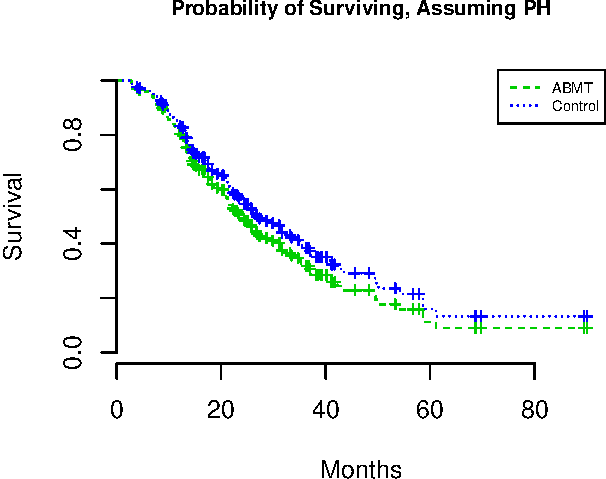
\includegraphics{unit_04_ph_reg_basics_files/figure-beamer/unnamed-chunk-16-1.pdf}

\end{frame}

\begin{frame}{%
\protect\hypertarget{example-pbt01-1}{%
Example: PBT01}}

Plot the estimated survival functions, by treatment, for each of the two
strata defined by cycle of response.

\begin{itemize}
\tightlist
\item
  Assuming a proportional hazards effect for ABMT
\end{itemize}

\end{frame}

\begin{frame}[fragile]{%
\protect\hypertarget{example-pbt01-2}{%
Example: PBT01}}

\scriptsize

\begin{Shaded}
\begin{Highlighting}[]
\KeywordTok{library}\NormalTok{(survival)}
\KeywordTok{library}\NormalTok{(eventtimedata)}
\KeywordTok{data}\NormalTok{(}\StringTok{"pbt01"}\NormalTok{)}

\NormalTok{pbt01.ph =}\StringTok{ }\KeywordTok{coxph}\NormalTok{(}\KeywordTok{Surv}\NormalTok{(survival,died) }\OperatorTok{~}\StringTok{ }\NormalTok{treatment }\OperatorTok{+}\StringTok{ }\KeywordTok{strata}\NormalTok{(cycle.of.resp),}
              \DataTypeTok{data =}\NormalTok{ pbt01)}
\NormalTok{newdata =}\StringTok{ }\KeywordTok{data.frame}\NormalTok{(}\DataTypeTok{treatment =} \KeywordTok{c}\NormalTok{(}\StringTok{"abmt"}\NormalTok{, }\StringTok{"control"}\NormalTok{))}

\NormalTok{\{}\KeywordTok{plot}\NormalTok{(}\KeywordTok{survfit}\NormalTok{(pbt01.ph, newdata), }\DataTypeTok{xlab =} \StringTok{"Months"}\NormalTok{, }\DataTypeTok{ylab=}\StringTok{"Survival"}\NormalTok{, }
     \DataTypeTok{lty =} \KeywordTok{c}\NormalTok{(}\DecValTok{2}\NormalTok{,}\DecValTok{2}\NormalTok{,}\DecValTok{3}\NormalTok{,}\DecValTok{3}\NormalTok{), }\DataTypeTok{col =} \DecValTok{3}\OperatorTok{:}\DecValTok{4}\NormalTok{, }\DataTypeTok{mark.time =} \OtherTok{TRUE}\NormalTok{,}
     \DataTypeTok{axes =} \OtherTok{FALSE}\NormalTok{, }
     \DataTypeTok{main =} \StringTok{"Probability of Surviving, ABMT"}\NormalTok{,}
     \DataTypeTok{cex =} \FloatTok{0.6}\NormalTok{, }
     \DataTypeTok{cex.main =} \FloatTok{0.8}\NormalTok{)}
\KeywordTok{axis}\NormalTok{(}\DecValTok{1}\NormalTok{)}
\KeywordTok{axis}\NormalTok{(}\DecValTok{2}\NormalTok{)}

\KeywordTok{legend}\NormalTok{(}\StringTok{"topright"}\NormalTok{, }\DataTypeTok{lty =} \KeywordTok{c}\NormalTok{(}\DecValTok{2}\NormalTok{,}\DecValTok{2}\NormalTok{,}\DecValTok{3}\NormalTok{,}\DecValTok{3}\NormalTok{), }\DataTypeTok{col =} \DecValTok{3}\OperatorTok{:}\DecValTok{4}\NormalTok{,}
       \KeywordTok{c}\NormalTok{(}\StringTok{"ABMT, resp cycle 1"}\NormalTok{, }\StringTok{"ABMT, resp cycle 2"}\NormalTok{,}
         \StringTok{"Control, resp cycle 1"}\NormalTok{, }\StringTok{"Control, resp cycle 2"}\NormalTok{),}
       \DataTypeTok{cex=}\FloatTok{0.6}\NormalTok{)}
\NormalTok{\}}
\end{Highlighting}
\end{Shaded}

\end{frame}

\begin{frame}

\scriptsize

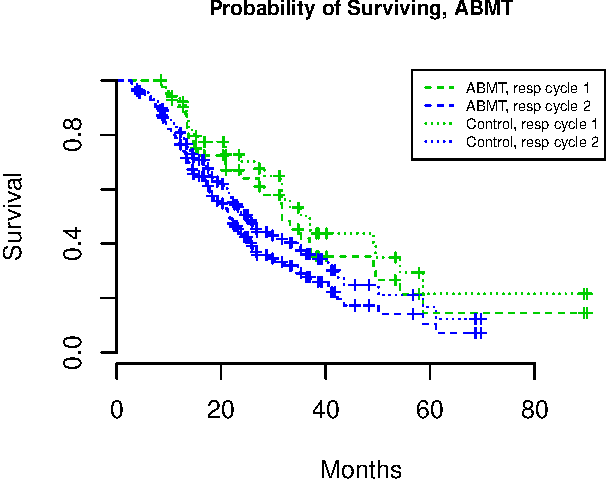
\includegraphics{unit_04_ph_reg_basics_files/figure-beamer/unnamed-chunk-18-1.pdf}

\end{frame}

\hypertarget{time-varying-time-dependent-covariates}{%
\section{Time-varying (time-dependent)
covariates}\label{time-varying-time-dependent-covariates}}

\begin{frame}{%
\protect\hypertarget{background-and-introduction}{%
Background and introduction}}

Conceptually (i.e., mathematically) there is little problem in extending
the \emph{PH} model to covariates that depend on time.

The model becomes \[
        \lambda(t;Z) = \lambda_0(t) \exp[\beta Z(t)]
\]

However, there can be problems in interpretation, especially when the
time-dependent covariate is essentially a surrogate for the event of
interest.

\end{frame}

\begin{frame}{%
\protect\hypertarget{issues-in-using-time-dependent-covariates}{%
Issues in using time-dependent covariates}}

The coding of the time-dependent covariate must be done with care.

\begin{itemize}
\item
  Software has not always been available. Robust routines are now
  available in \textsf{R} and \emph{SAS}.
\item
  The data structure required in \textsf{R} also works in \emph{SAS},
  but \emph{SAS} is more sometimes flexible.
\end{itemize}

This is best illustrated with an example: an intervention study in drug
addiction.\footnote{Hosmer and Lemeshow, \textit{Applied Survival Analysis}}

\end{frame}

\begin{frame}{%
\protect\hypertarget{example-umaru-impact-study-uis}{%
Example: UMARU Impact Study (UIS)}}

Data is from the University of Massachusetts AIDS Research Unit (UMARU)
IMPACT
Study.\footnote{Dataset \texttt{uis} in the package \texttt{eventtimedata}}

\begin{itemize}
\item
  5-year collaborative project comprised of two concurrent randomized
  trials of residential treatment for drug abuse

  \begin{itemize}
  \item
    \emph{Program A:} Randomized 444 subjects to a 3- or 6-month program
    of health education and relapse prevention. Clients taught to
    recognize “high-risk” situations that are triggers to relapse, and
    taught skills to cope with these situations without using drugs.
  \item
    \emph{Program B:} Randomized 184 participants to a 6- or 12-month
    program with highly structured lifestyle in a communal living
    setting.
  \end{itemize}
\item
  628 participants total
\end{itemize}

\end{frame}

\begin{frame}{%
\protect\hypertarget{variables-in-uis}{%
Variables in uis}}

\begin{tabular}{ll}
 \texttt{id} &  Subject ID (1-628)\\
 \texttt{age} &  Age in years\\
 \texttt{beck} &  Beck depression score\\
 \texttt{hercoc} &  Heroine or cocaine use prior to entry\\
 \texttt{ivhx} &  IV Drug use at admission\\
 \texttt{ndrugtx} &  Number of previous drug treatments\\
 \texttt{race} &  Race (white, other)\\
 \texttt{treat} &  Treatment assignment (short vs long)\\
 \texttt{site} &  Treatment program \\
 \texttt{los} &  Length of stay in Treatment (days)\\
 \texttt{time} &  Time to return to drug use (days)\\
 \texttt{censor} &  Indicator of drug use relapse (1 = yes, 0 = censored)
\end{tabular}

Details about coding in package documentation.

\end{frame}

\begin{frame}[fragile]{%
\protect\hypertarget{an-initial-model-for-uis}{%
An initial model for uis}}

Initial model estimates treatment effect, adjusting for

\begin{itemize}
\tightlist
\item
  Beck depression score, age, and race
\item
  interaction between age and site
\item
  interaction between race and site
\end{itemize}

\begin{Shaded}
\begin{Highlighting}[]
\KeywordTok{library}\NormalTok{(survival)}
\KeywordTok{library}\NormalTok{(eventtimedata)}
\KeywordTok{coxph}\NormalTok{(}\DataTypeTok{formula =} \KeywordTok{Surv}\NormalTok{(time, censor) }\OperatorTok{~}\StringTok{ }\NormalTok{treat }\OperatorTok{+}\StringTok{ }\NormalTok{beck }\OperatorTok{+}
\NormalTok{age }\OperatorTok{*}\StringTok{ }\NormalTok{site }\OperatorTok{+}\StringTok{ }\NormalTok{race }\OperatorTok{*}\StringTok{ }\NormalTok{site, }\DataTypeTok{data =}\NormalTok{ uis)}
\end{Highlighting}
\end{Shaded}

Model interpretation discussed with the next slide

\end{frame}

\begin{frame}[fragile]{%
\protect\hypertarget{an-initial-model-for-uis-1}{%
An initial model for uis\ldots}}

\footnotesize

\begin{verbatim}
## Call:
## coxph(formula = Surv(time, censor) ~ treat + beck + age * site + 
##     race * site, data = uis)
## 
##                     coef exp(coef) se(coef)     z       p
## treatlong       -0.26477   0.76738  0.09319 -2.84 0.00449
## beck             0.00975   1.00979  0.00481  2.03 0.04259
## age             -0.02369   0.97658  0.00934 -2.54 0.01116
## siteB           -1.10047   0.33271  0.52611 -2.09 0.03646
## raceother       -0.51190   0.59936  0.12988 -3.94 8.1e-05
## age:siteB        0.02441   1.02471  0.01602  1.52 0.12760
## siteB:raceother  0.80733   2.24191  0.24520  3.29 0.00099
## 
## Likelihood ratio test=37.2  on 7 df, p=4.29e-06
## n= 585, number of events= 471 
##    (43 observations deleted due to missingness)
\end{verbatim}

\normalsize

\end{frame}

\begin{frame}{%
\protect\hypertarget{what-is-the-effect-of-coming-off-treatment}{%
What is the effect of coming off treatment?}}

Hosmer, Lemeshow, and May speculated that the the important effect may
simply be stopping treatment, regardless of whether treatment is long or
short.

\begin{itemize}
\tightlist
\item
  Natural to look at the association between outcome and a
  time-dependent covariate that records when a patient stops treatment
\end{itemize}

The variable \texttt{treat.off} will take values

\begin{itemize}
\item
  0 while a subject is on treatment
\item
  1 starting at the time treatment stops
\end{itemize}

\end{frame}

\begin{frame}{%
\protect\hypertarget{time-dependent-covariates-in-r}{%
Time-dependent covariates in R}}

The work for time-dependent covariates in \textsf{R} is done in the data
structure.

If a covariate changes value over time, each case in the dataset should
have a row for each interval in which the covariate is constant. Each
row contains

\begin{itemize}
\item
  All fixed covariates and the outcome
\item
  Two variables that indicate the start (usually labeled \emph{tstart})
  and stop time (labeled \emph{tstop}) for that interval
\item
  The value of the time-dependent covariate in that interval
\end{itemize}

\end{frame}

\begin{frame}[fragile]{%
\protect\hypertarget{uis-data-with-time-dependent-variable-for-treatment}{%
UIS data with time-dependent variable for treatment}}

\footnotesize

\begin{verbatim}
##   id age beck los time censor tstart tstop relapse treat.off
## 1  1  39    9 123  188      1      0   123       0         0
## 2  1  39    9 123  188      1    123   188       1         1
## 3  2  33   34  25   26      1      0    25       0         0
## 4  2  33   34  25   26      1     25    26       1         1
## 5  3  33   10   7  207      1      0     7       0         0
## 6  3  33   10   7  207      1      7   207       1         1
## 7  4  32   20  66  144      1      0    66       0         0
## 8  4  32   20  66  144      1     66   144       1         1
\end{verbatim}

\normalsize

Original file has one row per case.

Code to create this file coming later.

\end{frame}

\begin{frame}[fragile]{%
\protect\hypertarget{two-models-involving-only-treatment}{%
Two models, involving only treatment}}

\scriptsize

\begin{verbatim}
## Call:
## coxph(formula = Surv(time, censor) ~ treat, data = uis)
## 
##             coef exp(coef) se(coef)    z      p
## treatlong -0.232     0.793    0.089 -2.6 0.0092
## 
## Likelihood ratio test=6.78  on 1 df, p=0.00921
## n= 628, number of events= 508
\end{verbatim}

\vspace{0.5cm}

\begin{verbatim}
## Call:
## coxph(formula = Surv(tstart, tstop, relapse) ~ treat * treat.off, 
##     data = uis2)
## 
##                       coef exp(coef) se(coef)     z      p
## treatlong           -0.523     0.593    0.226 -2.32  0.020
## treat.off            2.280     9.780    0.187 12.21 <2e-16
## treatlong:treat.off  0.621     1.861    0.246  2.52  0.012
## 
## Likelihood ratio test=389  on 3 df, p=0
## n= 1174, number of events= 508
\end{verbatim}

\end{frame}

\begin{frame}[fragile]{%
\protect\hypertarget{code-to-create-time-dependent-covariate-and-fit-models}{%
Code to create time-dependent covariate and fit models}}

\footnotesize

\begin{Shaded}
\begin{Highlighting}[]
\KeywordTok{library}\NormalTok{(survival)}
\KeywordTok{library}\NormalTok{(eventtimedata)}
\KeywordTok{data}\NormalTok{(}\StringTok{"uis"}\NormalTok{)}

\CommentTok{#model 1: original dataset}
\KeywordTok{coxph}\NormalTok{(}\KeywordTok{Surv}\NormalTok{(time, censor) }\OperatorTok{~}\StringTok{ }\NormalTok{treat, }\DataTypeTok{data =}\NormalTok{ uis)}

\CommentTok{#create file for time-dependent covariate}
\NormalTok{uis.temp =}\StringTok{ }\KeywordTok{tmerge}\NormalTok{(uis, uis, }\DataTypeTok{id =}\NormalTok{ id, }\DataTypeTok{relapse =} \KeywordTok{event}\NormalTok{(time, censor))}
\NormalTok{uis2 =}\StringTok{ }\KeywordTok{tmerge}\NormalTok{(uis.temp, uis.temp, }\DataTypeTok{id=}\NormalTok{id, }\DataTypeTok{treat.off =} \KeywordTok{tdc}\NormalTok{(los))}

\CommentTok{#model 2: time-dependent covariate}
\KeywordTok{coxph}\NormalTok{(}\KeywordTok{Surv}\NormalTok{(tstart, tstop, relapse) }\OperatorTok{~}\StringTok{ }\NormalTok{treat}\OperatorTok{*}\NormalTok{treat.off, }\DataTypeTok{data =}\NormalTok{ uis2)}
\end{Highlighting}
\end{Shaded}

\end{frame}

\begin{frame}[fragile]{%
\protect\hypertarget{a-larger-model}{%
A larger model}}

\footnotesize

\begin{verbatim}
## Call:
## coxph(formula = Surv(tstart, tstop, relapse) ~ treat * treat.off + 
##     beck + age + race + strata(site), data = uis2)
## 
##                         coef exp(coef) se(coef)     z       p
## treatlong           -0.53187   0.58751  0.24247 -2.19 0.02827
## treat.off            2.24928   9.48089  0.19729 11.40 < 2e-16
## beck                 0.00927   1.00931  0.00474  1.95 0.05076
## age                 -0.00291   0.99710  0.00747 -0.39 0.69729
## raceother           -0.41081   0.66311  0.11133 -3.69 0.00022
## treatlong:treat.off  0.68670   1.98715  0.26391  2.60 0.00927
## 
## Likelihood ratio test=370  on 6 df, p=0
## n= 1099, number of events= 471 
##    (75 observations deleted due to missingness)
\end{verbatim}

\end{frame}

\begin{frame}{%
\protect\hypertarget{coding-time-dependent-covariates}{%
Coding time-dependent covariates}}

The function \texttt{tmerge} works in many situations. See the
\href{../../methods_papers/t_therneau_time_dependent.pdf}{\textcolor{darkblue}{R vignette}}.
by Therneau, Crowson and Atkinson for additional examples.

\href{../../methods_papers/j_fox_rossi_time_dependent.pdf}{\textcolor{darkblue}{Fox}}
shows \textsf{R} code for the Rossi dataset, converting from a
wide-format to the long-format required by \textsf{R} for the monthly
employment status variable.

\end{frame}

\begin{frame}{%
\protect\hypertarget{partial-likelihood-with-time-varying-covariates}{%
Partial likelihood with time-varying covariates}}

Suppose there are \(K\) distinct failure times

\begin{itemize}
\item
  Let (\(\tau_1, \ldots, \tau_K\)) represent the \(K\) ordered, distinct
  death times. For now, assume there are no tied death times.
\item
  Let \({\cal R}(t) = \{ i: x_i \ge t \}\) denote the set of individuals
  who are at risk for failure at time \(t\).
\item
  Let \(i_j\) denote the label or identity of the individual who fails
  at time \(\tau_j\), including the value of his/her time-varying
  covariate during their time in the study
  \[   \{Z_{i_j}(t), t\in [0,\tau_j]\} \]
\item
  Let \(H_j\) denote the history of the entire data set, up to the
  \(j\)-th death or failure time, including the \emph{time} of the
  failure, but not the identity of the case who fails, also including
  the values of all covariates for everyone up to and including time
  \(\tau_j\).
\end{itemize}

\end{frame}

\begin{frame}{%
\protect\hypertarget{partial-likelihood-with-time-varying-covariates-1}{%
Partial likelihood with time-varying covariates\ldots}}

The partial likelihood in this setting can be written as \[
L(\bbeta) = \prod_{j=1}^{d} \frac {\exp(\bbeta {\bf Z}_{jj}) }
{\sum_{\ell \in {\cal R}(\tau_j)} \exp(\bbeta {\bf Z}_{\ell j}) },
\] where \({\bf Z}_{\ell j}\) is a way to denote the value of the
covariate vector for the \(\ell\)-th person at the \(j\)-th death time,
i.e. \[ {\bf Z}_{\ell j} =  {\bf Z}_\ell(\tau_j) \]

Inference proceeds similarly as in the standard case. The main
difference is that the values of \({\bf Z}\) changes at each risk set.

\end{frame}

\hypertarget{derivations}{%
\section{Derivations}\label{derivations}}

\begin{frame}{%
\protect\hypertarget{additional-derivation-of-the-partial-likelihood}{%
Additional derivation of the partial likelihood}}

In general, the likelihood contributions for censored data fall into two
categories:

\begin{itemize}
\item
  \emph{Individual is censored at \(X_i\):}
  \[L_i(\beta)= S(X_i) = \exp[-\int_0^{X_i} \lambda_i(u)du]\]
\item
  \emph{Individual fails at \(X_i\):}
  \[L_i(\beta)= S(X_i) \lambda_i(X_i) = \lambda_i(X_i) \exp[-\int_0^{X_i} \lambda_i(u)du]\]
\end{itemize}

Thus, everyone contributes \(S(X_i)\) to the likelihood, and only those
who fail contribute \(\lambda_i(X_i)\).

\end{frame}

\begin{frame}{%
\protect\hypertarget{additional-derivation-of-the-partial-likelihood-1}{%
Additional derivation of the partial likelihood \ldots}}

The total likelihood will be : \begin{align*}
L(\beta) &= \prod_{i=1}^n \lambda_i(X_i)^{\delta_i} \;
\exp[-\int_0^{X_i} \lambda_i(u)du]
\end{align*}

The above likelihood holds for all censored survival data, with general
hazard function \(\lambda(t)\).

It does not depend on the PH assumption.

\end{frame}

\begin{frame}{%
\protect\hypertarget{additional-derivation-of-the-partial-likelihood-2}{%
Additional derivation of the partial likelihood \ldots}}

Now multiply and divide by the term
\(\left[\sum_{j\in {\cal R}(X_i)} \lambda_i(X_i)\right]^{\delta_i}\):

\begin{align*}
L(\beta) &= \prod_{i=1}^n \left[\frac{\lambda_i(X_i)}{\sum_{j\in {\cal R}(X_i)}\lambda_i(X_i)}\right]^{\delta_i} \; 
\left[\sum_{j\in {\cal R}(X_i)} \lambda_i(X_i)\right]^{\delta_i} \;
\exp[-\int_0^{X_i} \lambda_i(u)du]
\end{align*}

Cox (1972) argued that the first term in this product contains almost
all the information about \(\beta\), while the last two terms contain
information about the baseline hazard \(\lambda_0(t)\).

\end{frame}

\begin{frame}{%
\protect\hypertarget{additional-derivation-of-the-partial-likelihood-3}{%
Additional derivation of the partial likelihood \ldots}}

Under the Cox PH assumption, the first term can be written as
\begin{align*}
L(\bbeta) &= \prod_{i=1}^n \left[\frac{\lambda_i(X_i)}{\sum_{j\in
{\cal R}(X_i)}\lambda_i(X_i)}\right]^{\delta_i}\\
&=\prod_{i=1}^n \left[ \frac{\lambda_0(X_i)\exp(\beta {\bf Z}_i)}
{\sum_{j\in {\cal R}(X_i)}
\lambda_0(X_i)\exp(\bbeta {\bf Z}_j)}\right]^{\delta_i}\\
&=\prod_{i=1}^n \left[ \frac{\exp(\bbeta {\bf Z}_i)}
{\sum_{j\in {\cal R}(X_i)}\exp(\bbeta {\bf Z}_j)}\right]^{\delta_i}
\end{align*}

This is the partial likelihood defined by Cox; it does not depend on the
underlying hazard \(\lambda_0(\cdot)\).

Cox recommended treating this as an ordinary likelihood for making
inferences about \(\beta\) in the presence of the nuisance parameter
\(\lambda_0(\cdot)\).

\end{frame}

\end{document}
